\chapter{Experiments}\label{ch:experiments}
In this chapter we will exploit in detail some experiments performed over the RAW Dataset presented in Chatper \ref{ch:raw_dataset}. In particular we will first focus on some object detection experiments performed both with standard shape based approaches as described in Sec. \ref{subsec:template_matching} and deep learning based approaches as described in Sec. \ref{subsec:dl_obj_detection}. Moreover, we will exploit the results of our implementation of the SGM algorithm described in Sec. \ref{subsec:semiglobalmatching} comparing its results with the ground truth depth image created by reconstructing the 3D scene with the ground truth objects pose obtained with the labeling procedure described in Sec. \ref{sec:ground_truth_estim}.

%\section{Region Proposal}\label{sec:exp_region_proposal}
%To do ...

\section{Object Detection}\label{sec:exp_object_detection}
As aleady inoduced in Sec. \ref{sec:objectdetection}, object detection is basically the task of computing the 2D boinging box of a given object within an image. Bounding box is essentially a portion of the image that contains the object. Such basic information is extremely important in robotic perception, especially in robotic vision, where the ability to detect objects in different situations is a crucial point. Our tests basically rely on testing the performances of two different kind of approaches, namely shape based and deep learning.

The tests have been performed on a subset of the RAW Dataset, since the availability of the ground truth for the entire dataset has not been achieved yet, moreover it is not part of the scope of this work. The subset of the RAW Dataset is anyway enough large to permit consistent and coherent statistical evaluations, and it is composed as follows:

\begin{itemize}
	\item \textbf{2 complete scenes}: the tests have been performed using just the first two scenes of the dataset, and just with respect to the data obtained from the experimental FlexSight Sensor, as its performance evaluation is a consistent and important part of the FlexSight project (See Appendix \ref{apx:flexsight});
	\item \textbf{Almost 4 thousand of images}: the two scenes contains both camera left and camera right of the FlexSight Sensor, both with and without projected laser pattern;
	\item \textbf{All the images are labeled}: all the considered images have are accompanied with the relative ground truth 3D position of each object and the relative bounding box as well;
	\item \textbf{5 Different Object Classes}: the involved images only contain 5 object classes of the RAW Dataset, namely: \emph{Distance\_tube}, \emph{M20}, \emph{M20\_100}, \emph{Cover\_plate\_BOX}, \emph{S40\_40\_G};
	\item \textbf{Synthetic data generation}: for the deep learning approaches, data augmentation has been employed. In particular we will see in the following subsections how we trained the YOLO deep neural network described in Sec. \ref{subsec:dl_obj_detection} with 2 different version of the RAW Dataset subset, namely the first is the original one and the second is a synthetic version of it.
\end{itemize}

The results wiil be organized by class of the object and will be expressed in terms of IoU accuracy over the detected bounding box.

\subsection{Shape Based Approach Results - Halcon object detection}\label{subsec:halcon_obj_det_results}
\subsubsection{Experiment Details}
In this experiment, we performed both object localization and detection since the core of the object detection pipeline of the Halcon libs is essentially based on 3D object localization on 2D images, then given the 3D position of the object w.r.t. the camera frame, it is projected onto the 2D image and the bounding box of the object is extracted. Examples of this procedure is given in \figref{fig:iou_example}. Moreover, given the highly customization level that those library has, we investigated object detection performances by considering multiple settings:

\begin{itemize}
	\item \textbf{Single object candidate detection}: Only the object with the highest score is considered;
	\item \textbf{Multiple object candidates detection}: We analyzed both the performances using in sequence: \emph{5 candidates}, \emph{4 candidates}, \emph{3 candidates} and \emph{2 candidates}.
\end{itemize}

\begin{figure}
    \centering
    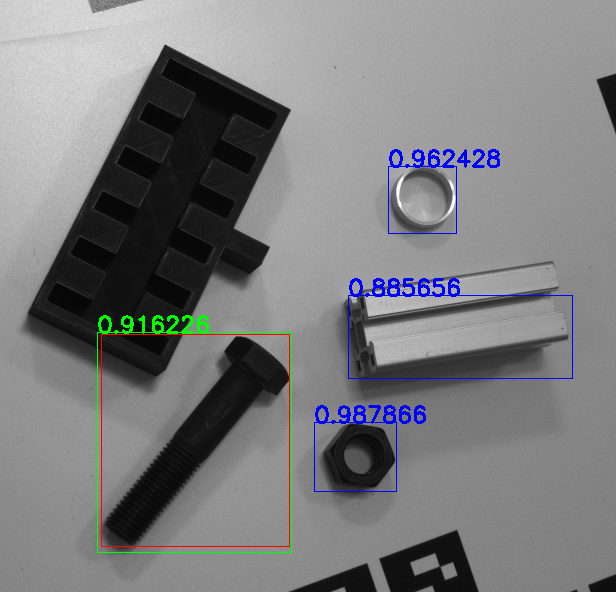
\includegraphics[width=0.8\textwidth]{figures/4_experiments/m20_100_halcon_detection_problems}
    \caption{\textbf{Best Candidate Problems with Halcon Libraries}. The picture depicts an example of erroneous best candidate detection. The candidate that actually refers to the real M20\_100 object is not the one with the highest score. In a single candidate approach the detection would have failed.}
    \label{fig:m20_100_halcon_detection_problems}
\end{figure}

\subsubsection{Experiment Results}
As already anticipated, each result will be presented differentiating for each class of the considered objects. The \tabref{tab:big_table_results} show the accuracy results in terms of Intersection over Union (IoU) for each of the involved object, look at the section referred to Shape Based Approach.

As expected, the performances slightly increase when including in the search procedure the highest number of candidates. That is essentially due to the fact that not always the first best candidate, namely the object with the highest score, is exactly the object that we are looking for. If we compare more than one candidate with the ground truth bounding box we find that for some classes of objects, like the \emph{M20\_100}, only when we consider 5 candidates we achieve to detect the actual object, and even in such cases, the one that has the highest score is not the right object (See. \figref{fig:m20_100_halcon_detection_problems} for a better visualization of the described problem).

\begin{table}[ht!]
 \centering

   \begin{tabular}{ llllllll }
   &\multicolumn{5}{c}{ \textbf{Shape Based} } &\multicolumn{2}{c}{ \textbf{Deep Learning} }\\
   \cmidrule(lr){2-6} \cmidrule(lr){7-8}
   \textbf{Obj Class} & \emph{1Cand} & \emph{2Cand} & \emph{3Cand} &\emph{4Cand} & \emph{5Cand} & $YOLO_O$ & $YOLO_S$\\
   \cmidrule(lr){1-8}   
   \emph{Distance\_tube} & 0.862 & 0.862 & 0.862 & 0.862 & 0.862 & \cellcolor{gray!25}0.897 & 0.825 \\ 
   \emph{M20} & 0.744 & 0.744 & 0.746 & 0.746 & 0.746 & \cellcolor{gray!25}0.901 & 0.816 \\ 
   \emph{M20\_100} & 0.000 & 0.000 & 0.475 & 0.475 & 0.797 & \cellcolor{gray!25}0.944 & 0.890 \\
   \emph{Cover\_plate\_BOX} & 0.799 & 0.799 & 0.799 & 0.799 & 0.799 & \cellcolor{gray!25}0.954 & 0.921 \\
   \emph{S40\_40\_G} & 0.809 & 0.809 & 0.809 & 0.809 & 0.809 & \cellcolor{gray!25}0.939 & 0.829 \\
%   \vspace{0.025cm} \\
%   \cline{1-8} \\
   \end{tabular} 
   \caption{\textbf{IoU Average results}: the table reports the results in terms of IoU Average (Intersection over Union Average) of all the tested methods. Results are reported by object class organized in columns by Shape Based Approach and Deep Learning Approach. Shape Based Approach results are reported by number of candidates used for the detection.}
 \label{tab:big_table_results}
\end{table}

%\begin{table}[!hbt]
%\parbox{.45\linewidth}{
%	\centering
%    \begin{tabular}{| l | l |}
%    \hline
%    \textbf{Experiment Type} & \textbf{IoU Average} \\ \hline
%    \emph{5 candidates} & 0.86190 \\
%    \emph{4 candidates} & 0.86190 \\
%    \emph{3 candidates} & 0.86190 \\
%    \emph{2 candidates} & 0.86190 \\
%    \emph{1 candidate} & 0.86190 \\
%    \hline
%    \end{tabular}
%    \caption{\textbf{Halcon IoU avg. scores on Distance\_tube object.}}
%    \label{tab:halcon_distance_tube_results}
%}
%\hfill
%\parbox{.45\linewidth}{
%	\centering
%    \begin{tabular}{| l | l |}
%    \hline
%    \textbf{Experiment Type} & \textbf{IoU Average} \\ \hline
%    \emph{5 candidates} & \textbf{0.74614} \\
%    \emph{4 candidates} & \textbf{0.74614} \\
%    \emph{3 candidates} & \textbf{0.74614} \\
%    \emph{2 candidates} & 0.74418\\
%    \emph{1 candidate} & 0.74418\\
%    \hline
%    \end{tabular}
%    \caption{\textbf{Halcon IoU avg. scores on M20 object.}}
%    \label{tab:halcon_M20_results}
%}
%\end{table}
%
%\begin{table}[!hbt]
%\parbox{.45\linewidth}{
%	\centering
%    \begin{tabular}{| l | l |}
%    \hline
%    \textbf{Experiment Type} & \textbf{IoU Average} \\ \hline
%    \emph{5 candidates} & \textbf{0.79750} \\
%    \emph{4 candidates} & 0.47585 \\
%    \emph{3 candidates} & 0.47585 \\
%    \emph{2 candidates} & 0.00000 \\
%    \emph{1 candidate} & 0.00000 \\
%    \hline
%    \end{tabular}
%    \caption{\textbf{Halcon IoU avg. scores on M20\_100 object.}}
%    \label{tab:halcon_M20_100_results}
%}
%\hfill
%\parbox{.45\linewidth}{
%	\centering
%    \begin{tabular}{| l | l |}
%    \hline
%    \textbf{Experiment Type} & \textbf{IoU Average} \\ \hline
%    \emph{5 candidates} & \textbf{0.79978} \\
%    \emph{4 candidates} & \textbf{0.79978} \\
%    \emph{3 candidates} & \textbf{0.79978} \\
%    \emph{2 candidates} & \textbf{0.79978} \\
%    \emph{1 candidate} & 0.12 \\
%    \hline
%    \end{tabular}
%    \caption{\textbf{Halcon IoU avg. scores on Cover\_plate\_BOX object.}}
%    \label{tab:halcon_Cover_plate_BOX_results}
%}
%\end{table}
%
%\begin{table}[!hbt]
%	\centering
%    \begin{tabular}{| l | l |}
%    \hline
%    \textbf{Experiment Type} & \textbf{IoU Average} \\ \hline
%    \emph{5 candidates} & 0.80922 \\
%    \emph{4 candidates} & 0.80922 \\
%    \emph{3 candidates} & 0.80922 \\
%    \emph{2 candidates} & 0.80922 \\
%    \emph{1 candidate} & 0.80922 \\
%    \hline
%    \end{tabular}
%    \caption{\textbf{Halcon IoU avg. scores on S40\_40\_G object.}}
%    \label{tab:halcon_S40_40_G_results}
%\end{table}

\subsection{Deep Learning Approach Results - YOLO}\label{subsec:yolo_obj_det_results}
\subsubsection{Experiment Details}
Deep learning is become one of the prominent and more prolific area of research in the last decade, and latest techniques and developments have actually now reached the state-of-the-art in many tasks. Object detection is one of them. That is why we wished to test some of those techniques, e.g. YOLO deep neural network, and compare its performance w.r.t. the technique used in the last experiment. In this experiment we are going to show multiple results of YOLO object detection capabilities and explain how we achieved higher levels of IoU Avg. detection rate w.r.t. the Halcon libraries.

The experiment has been conducted using almost the very same settings of the previous experiment, with just few modifications in order to be compliant with this totally different approach. In particular, given the data driven nature of this approach we must subdivide the dataset in two different sets: \emph{training set}, \emph{evaluation set}. In particular we used $95\%$ of the initial subset as training set, and the remaining $5\%$ as validation set. The high disparity among the two set sizes is simply because such approaches need lot of data in order to be trained successfully, that is we gave almost all the subset to the training set. The validation set at the end is big enough to obtain reliable results ($\sim$ 100 images). From now on, we will refer to this version of the dataset as \emph{$YOLO_O$}, as it is directly built from the original RAW Dataset, and just adapted to the YOLO format. The same acronym will be given to the related network as well.

\begin{table}
	\centering
    \begin{tabular}{| l | l |}
    \hline
    \textbf{Parameter} & \textbf{Value} \\ \hline
    \emph{batch size} & 64 \\
	\emph{height} & 416 \\
	\emph{momentum} & 0.9 \\
	\emph{decay} & 0.0005 \\
	\emph{learning rate} & 0.0001 \\
	\emph{max batches} & 15000 \\
	\emph{policy} & steps \\
	\emph{steps} & 100, 8000, 10500 \\
    \hline
    \end{tabular}
    \caption{\textbf{$YOLO_O$ training parameters.} In the table are reported the most significant parameters that we tuned in order to train the $YOLO_O$ network. All the others are assumed as with their default value.}
    \label{tab:YOLO_standard_training_params}
\end{table}

The training of the $YOLO_O$ network has been conducted using the set of parameters given in \tabref{tab:YOLO_standard_training_params}. With the very same set of parameters we performed another train of the YOLO network. In particular we used a \emph{synthetic} version of the RAW Dataset, from now on we will refer to it as $YOLO_S$, built by manipulating the same training images used for $YOLO_O$'s training. The basic idea was to change the background of all the images with random images downloaded from the publicly available set of images at the following site: \url{https://snippets.khromov.se/stock-photo-archive-zip-77-images/}. Some example of images realized with such technique, are given in \figref{fig:synthetic_dataset_ex}.

\begin{figure}
    \centering
    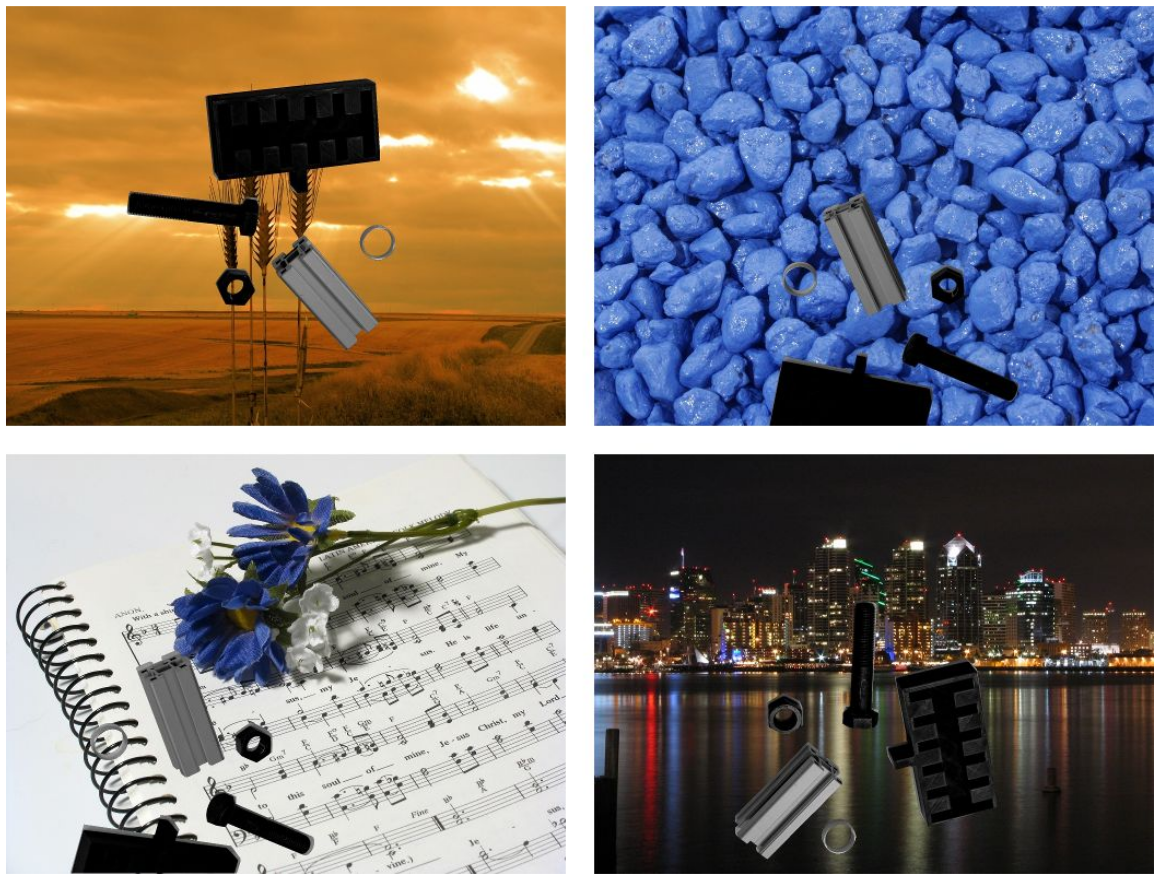
\includegraphics[width=0.8\textwidth]{figures/4_experiments/synthetic_dataset_ex}
    \caption{\textbf{Images from the synthetic RAW Dataset}. In the figure, some examples of the images produced for training the $YOLO_S$ network.}
    \label{fig:synthetic_dataset_ex}
\end{figure}
%\begin{table}
%	\centering
%    \begin{tabular}{| l | l | l |}
%    \hline
%    \textbf{Object Class} & \textbf{$\pmb{YOLO_O}$ - IoU Avg.} & \textbf{$\pmb{YOLO_S}$- IoU Avg.}\\ \hline
%    \emph{Distance\_tube} & \textbf{0.89749} & 0.82526 \\
%    \emph{M20} & \textbf{0.90142} & 0.81673 \\
%    \emph{M20\_100} & \textbf{0.94402} & 0.89050 \\
%    \emph{Cover\_plate\_BOX} & \textbf{0.95479} & 0.92168 \\
%    \emph{S40\_40\_G} & \textbf{0.93904} & 0.82985 \\
%    \hline
%    \end{tabular}
%    \caption{\textbf{YOLO Detection Results}: Both YOLO trained with original RAW Dataset ($YOLO_O$) and with the Synthetic generated dataset ($YOLO_S$).Those results are referred to test images of the original RAW Dataset, not the synthetic generated version.}
%    \label{tab:dl_YOLO_results_unified}
%\end{table}
\subsubsection{Experiment Details}
In the \textbf{Deep Learning} section of \tabref{tab:big_table_results} are reported some results of the test performed with the two networks, namely $YOLO_O$ and $YOLO_S$. The results have been arranged in the same way as the experiment shown before in order to give a comprehensive and consistent way for comparing the two approaches. It is clearly evident that the Deep Learning approaches overcome the shape based ones by more than $\sim10\%$. The main reason why we performed also this other kind of training is that the first network, the $YOLO_O$, seemed to be overfitting the dataset used for training, and the reasons are essentially two:

\begin{itemize}
	\item \textbf{Little size of the training set}: We used only a subset of the overall RAW Dataset, and maybe they are too few images for successfully such a big network (more than 20 convolutional layers + fully connected layers at the end);
	\item \textbf{Too similar images}: images used for the training phase are extremely similar, even if taken from completely different views. Illumination conditions are almost always the same, background is always the same, and so on.
\end{itemize}

We basically claim that such configuration brought the $YOLO_O$ network to overfitting a bit the training set, and clearly evidence of this is given by the result of the detection performed on very different scenes, with objects in a much more cluttered environment. Look at \figref{fig:overfitting_problem} for better understanding the problem. Results show that we overcome a bit the problem of overfitting with the network trained with the standard RAW Dataset.

\begin{figure}
    \centering
    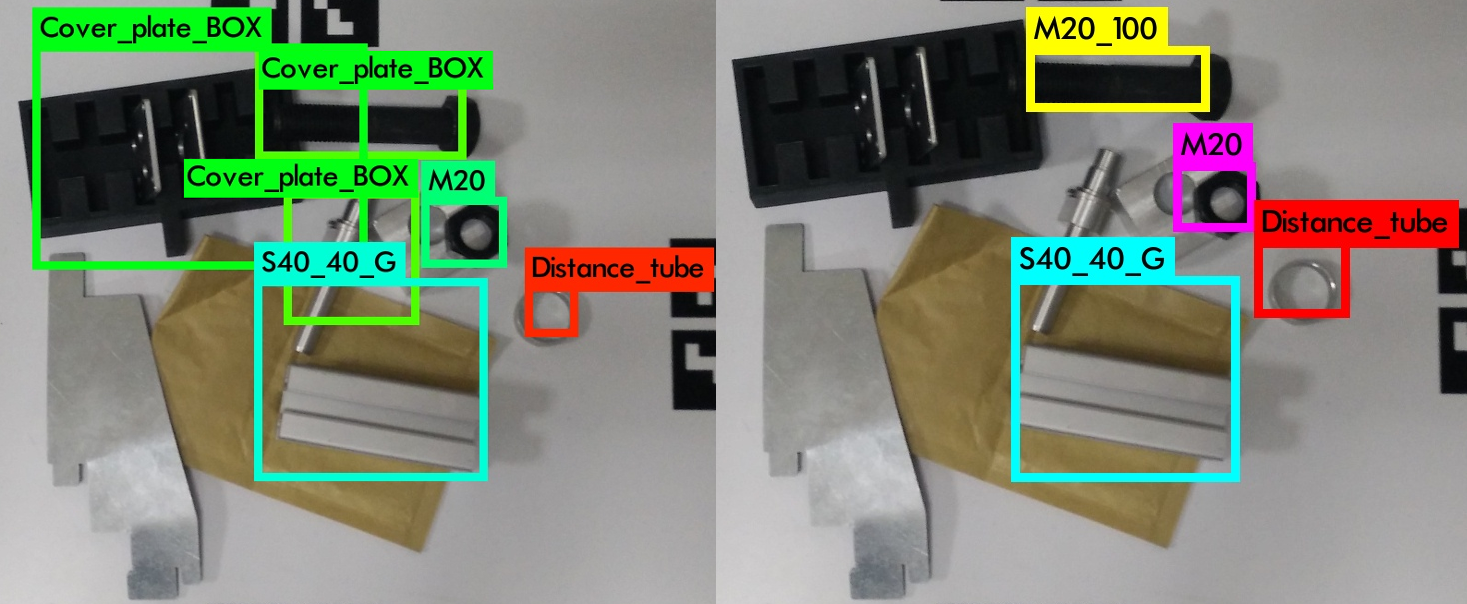
\includegraphics[width=\textwidth]{figures/4_experiments/overfitting_problem}
    \caption{\textbf{Detection Results on totally different scene}. The scene depicted in the image is taken ot of the RAW Dataset, is not part of it essentially. Was built for testing $YOLO_O$ and $YOLO_S$ performances out of the training and test set. On the left there is the result of $YOLO_O$'s detection, on the right the $YOLO_S$'s one. It is clearly evident that $YOLO_S$ is much more robust than the first one. So results show that we overcome a bit the problem of overfitting with the network trained with the standard RAW Dataset.}
    \label{fig:overfitting_problem}
\end{figure}

%\section{Stereo Matching}\label{sec:exp_stereo_matcing}
%To do ...

\section{3D Reconstruction}\label{sec:exp_3d_reconstruction}
To do ...

\section{Discussion}\label{sec:exp_discussion}
To do ...